\documentclass{standalone}
\usepackage{tikz}
\begin{document}
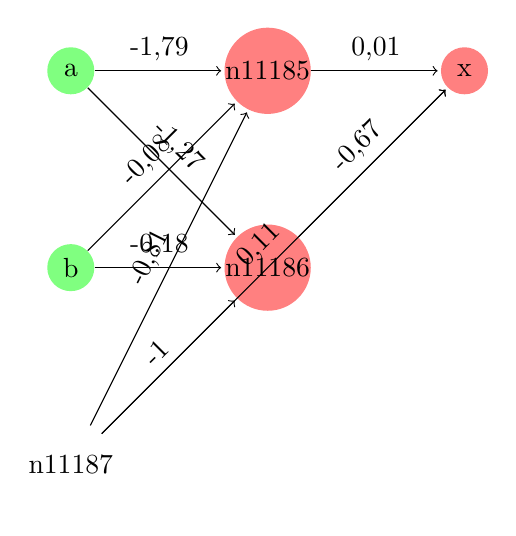
\begin{tikzpicture}[shorten >=1pt,->,draw=black!,node distance=2.5cm]
\tikzstyle{neuron}=[circle,fill=black!25,minimum size=17pt,inner sep=0pt]
\tikzstyle{constant}=[neuron, fill=white!50];
\tikzstyle{sigmoid}=[neuron, fill=red!50];
\tikzstyle{identity}=[neuron, fill=green!50];
\node [identity] (a) {a};
\node [identity,below of=a] (b) {b};
\node [constant,below of=b] (n11187) {n11187};
\node [sigmoid,right of=a] (n11185) {n11185};
\node [sigmoid,below of=n11185] (n11186) {n11186};
\node [sigmoid,right of=n11185] (x) {x};
\path[every node/.style={sloped,anchor=south,auto=false}]
(n11185) edge node {0,01} (x)
(n11186) edge node {-0,67} (x)
(b) edge node {-0,18} (n11186)
(b) edge node {-0,08} (n11185)
(a) edge node {-1,27} (n11186)
(a) edge node {-1,79} (n11185)
(n11187) edge node {0,11} (x)
(n11187) edge node {-1} (n11186)
(n11187) edge node {-0,81} (n11185)
;\end{tikzpicture}
\end{document}